\section{Introduction} \label{sec:intro}
Software systems evolve by nature \cite{lehman:1980}. The activity of software development becomes more complex as the system evolves, which leads to the need for preventive and corrective maintenance. This complexity is reflected in the fact that about 90\% of the total costs of software systems are associated with their maintenance \cite{erlikh:2000}. Therefore, the area represents a promising field for improvement.

Visualization techniques have been used in software engineering as a possible solution to the difficult task of understanding, maintaining and evolving software systems. The visual metaphors are very useful in this context because sight is the most developed sense in human being \cite{diehl:2007}.

During the last decade, tools such as CodeCity~\cite{wettel:2008} have used 3D visualizations to represent, and hopefully provide a better understanding of, software. 3D visualization is sometimes more intuitive and has an extra dimension that allows the visualization of a larger amounts of information in relation to 2D visualization \cite{teyseyre:2009}. However, it also has an important limitation. The computer screen is bi-dimensional and always occludes something that is represented three dimensionally. A solution to the problem of interaction between the user and 3D software is the use of augmented reality. This technology makes virtual objects visible in real environments, facilitating virtual interaction with the user, since the communication can be done through gestures and movements \cite{azuma:1997}.

This paper presents SkyscrapAR, a new software evolution visualization approach that uses a city metaphor combined with augmented reality techniques. SkyscrapAR represents software classes and packages as 3D buildings of a chosen project revision number. These buildings are laid over on a terrain baseline blueprint derived from all versions of the software project. Buildings are sized up and colored by their size and number of changes. The project revision displayed can be dynamically chosen and buildings can be dynamically filtered for better evolution analysis. The augmented reality approach allows for easy manipulation of the produced visual scenarios. To the best of our knowledge, there is no other work in the literature that uses this approach.

\todo{Review}This paper is structured as follows. Section 2 introduces related work. Section 3 presents SkyscrapAR and its features. Then, Section 4 discusses some applications of the tool. Finally, Section 5 concludes this article.

\section{SkyscrapAR} \label{sec:skyscrapar}
SkyscrapAR is an augmented reality (AR) software evolution visualization based on the metaphor of an evolving city. Similarly to CodeCity~\cite{wettel:2008}, SkyscrapAR represents packages (or folders in the source code file structure) as rectangular city lots, with sub-packages being stacked on top of the package containing them (see Figure~\ref{fig:sample_junit}). Classes (or source code implementation files) are represented by buildings (boxes with different areas and heights) located on top of their respective packages, with the area they occupy being proportional to the size of the class, measured in lines of code. The user can browse over revisions of the software, and see buildings appearing, disappearing, and changing their shape to reflect successive modifications that they suffered over time.

\begin{figure}[ht!]
 \centering
 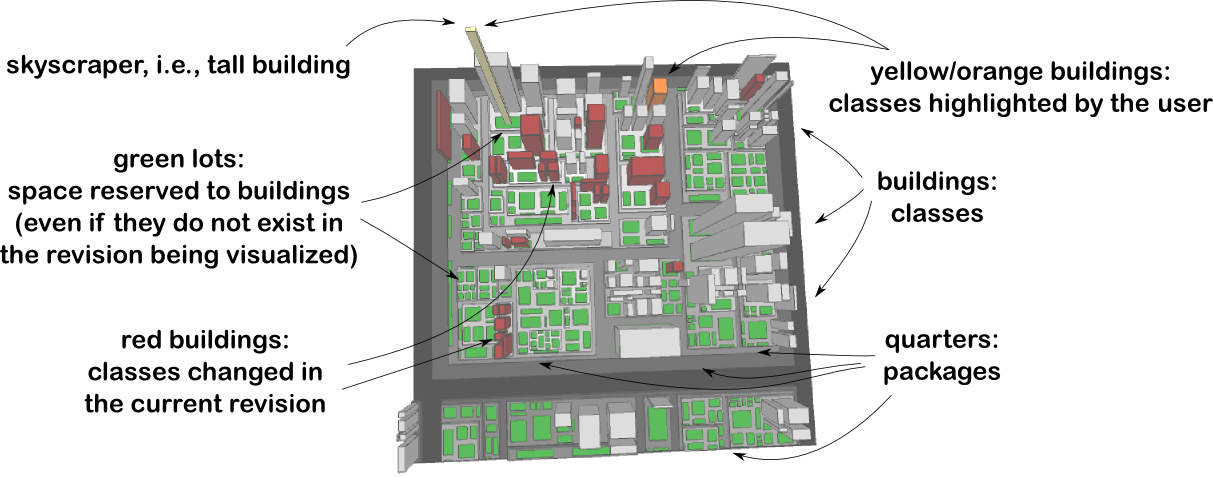
\includegraphics[width=0.5\textwidth, bb=0 0 1214 477]{./images/infographic}
 % fig1 - infographic.png: 1213x477 pixel, 72dpi, 42.82x16.84 cm, bb=0 0 1214 477
 \caption{The JUnit framework visualized as a city using SkyscrapAR.}
 \label{fig:sample_junit}
\end{figure}

Because the city (i.e., the software) evolves over time, it must have space to accommodate all buildings that existed in some period of its history. That is why the city terrain is divided in green lots, each one belonging to a building (i.e., a class). Green lots are large enough to fit their respective buildings when they reach maximum area. So, for example, buildings which present some green area in the last revision represent classes that used to be larger but had their size reduced.

The full source code is also publicly available under an open source license\footnote{\url{https://github.com/rodrigorgs/SkyscrapAR}}. The rest of this section describes SkyscrapAR in terms of its architecture, used source code metrics, and its user interface.

\subsection{Architecture} \label{sec:architecture}
SkyscrapAR is composed of two executables: the extractor and the viewer. The extractor, written in Java, reads a local Git repository containing Java source code and outputs a XML file describing its revisions, along with information for each source code file that was modified in each revision. The viewer, written in Processing\footnote{\url{http://processing.org/}}, takes the XML file and presents its data as a city that the user can view and interact with.

\begin{figure}[ht!]
 \centering
 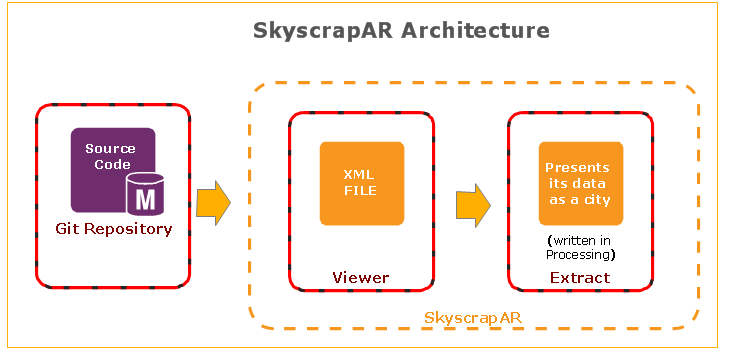
\includegraphics[width=0.5\textwidth, bb=0 0 547 269]{./images/architecture}
 % architecture.png: 729x359 pixel, 96dpi, 19.29x9.50 cm, bb=0 0 547 269
 \caption{SkyscrapAR architecture}
 \label{fig:architecture}
\end{figure}

The hardware setup needed to use the visualization is printed marker and a computer with screen and camera, as shown in Figure~\ref{fig:setup}. A marker is a piece of paper or any other object with a predefined black and white square pattern printed on it. The marker signals where the city will be rendered appear within the user’s environment. The user interacts with the visualization as he would do with a mock-up city, manipulating the marker with the hands so the city can be seen from the desired viewpoint.

\begin{figure}[h!]
 \centering
 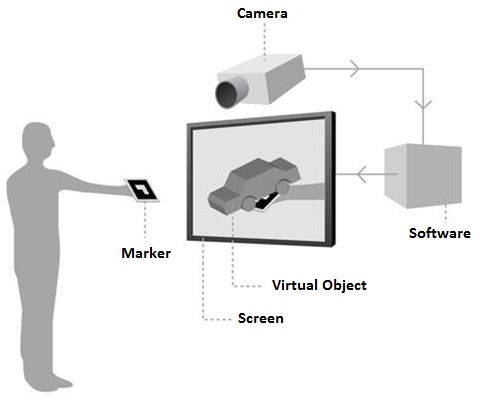
\includegraphics[width=0.4\textwidth, bb=0 0 486 406]{./images/howtowork.jpg}
 % howtowork.jpg: 479x400 pixel, 71dpi, 17.14x14.31 cm, bb=0 0 486 406
 \caption{Augmented reality setup.}
 \label{fig:setup}
\end{figure}

The processing needed for augmented reality is shown in Figure~\ref{fig:rendering_visualization}. Each frame captured by the camera is converted to a binary, black and white image, according to configurable brightness threshold. An algorithm then detects black square contours and then compares its inside with a predefined pattern. If they match, then it builds a local 3D coordinate system for the marker, as shown in Figure~\ref{fig:rendering_visualization}b. The 3D model of the city is then aligned with the local coordinate axes, as shown in Figure~\ref{fig:rendering_visualization}c, so it moves together with the marker, giving the effect that it is a part of the real world.

\begin{figure}[ht!]
 \centering
 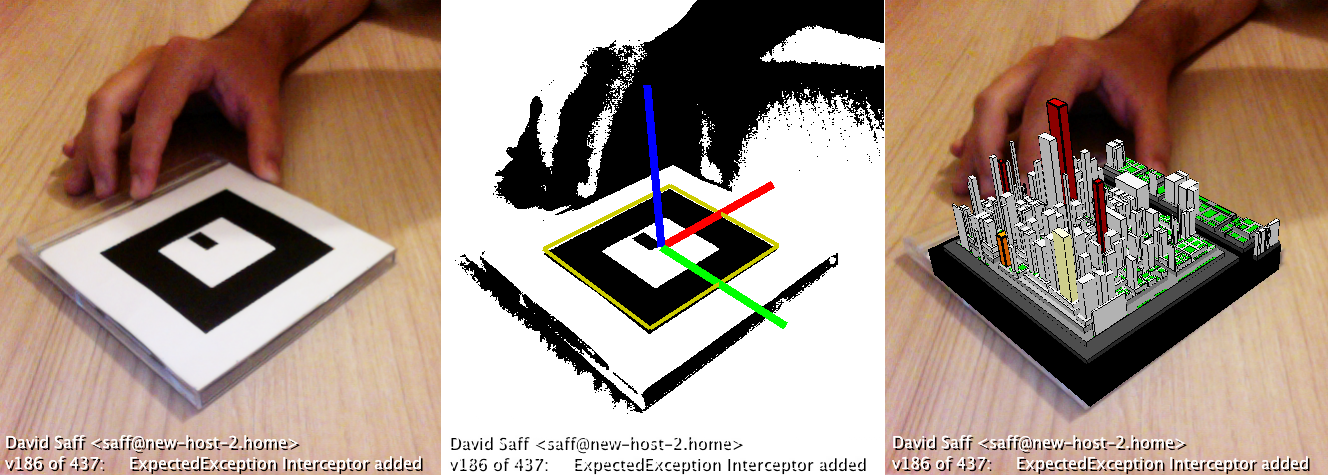
\includegraphics[width=0.5\textwidth, bb=14 14 1343 490]{./images/visualizationRedering}
 % visualizationRedering.eps: 0x0 pixel, 300dpi, 0.00x0.00 cm, bb=14 14 1343 490
 \caption{Rendering the visualization scene with augmented reality}
 \label{fig:rendering_visualization}
\end{figure}

\subsection{Mapping Metrics to Visual Elements} \label{sec:metrics_visual_elements}
A software system is composed of consecutive revisions. In each revision, two metrics are computed for all the classes: number of lines of code (LOC) and code churn. 

The LOC metric is the total number of lines in the respective source code file, including comments and blank lines. This metric, although simple to measure, correlates with many traditional complexity metrics that are used to predict development effort and fault proneness \cite{elemam:2001}.

Code churn refers to how much a particular file has been modified in its current and previous revisions in the version control system. The code churn of a class in its initial revision is equal to its LOC. Then, each time the class is modified, the code churn is incremented by the number of lines of code added or removed in the revision, as computed by Unix’s diff tool. That way, code churn always increases or is kept constant over time. The rationale for code churn is that source code files modified frequently are less stable and tend to be more prone to faults \cite{nagappan:2005}.

\subsection{User Interface} \label{sec:user_interface}
The user interface for SkyscrapAR displays the scene being captured by the camera and, if a marker is on the scene, the 3D model of the city is superimposed on it. In the bottom part of the screen, information about the current revision being visualized is displayed. It includes the sequential number of the revision, together with the name of the developer responsible for the change and the message describing the change.

Contrary to what happens in most 3D software visualizations, where users change their viewpoint by using the mouse or the keyboard, in SkyscrapAR, the user can view the city from different angles by manipulating either the 3D marker or the camera. With such interaction mechanism, the user can explore all six degrees of freedom of the 3D space (translation and rotation along three axes) in a natural way. For instance, the city can be seen from the top, in an aerial view, evidencing the structure of the software, or sideways, in a skyline view, evidencing skyscrapers, i.e., classes with high code churn.

In its current state, SkyscrapAR still depends on mouse and keyboard input, although we plan to reduce this dependency. The mouse pointer is used to highlight classes the user may want to focus on. The keyboard is mainly used to navigate through revisions, using the left and right arrow keys.

When the user advances the visualization to the next revision, buildings representing classes that were modified in that revision appear in red, so they can be easily spotted among the default gray buildings. It is expected that the buildings in red changed its shape compared to the previous revision 1 to reflect changes in the number of lines of code (area of the base) or in its code churn (height). Such changes in shape are presented as a smooth animation, by interpolating the dimensions of the buildings over a short period of time (less than one second). That way, it is easier to track the changes in the classes over time, enhancing the perception of evolution.

When the mouse pointer is over a building, the interface shows information for the respective class: name, package containing it, and the values for the LOC and code churn metrics. The user can also highlight a set of buildings, which get painted in yellow, by clicking on them. If a class is highlighted and has changed in the current revision, it gets painted in orange instead (i.e., a red and yellow mix). 

The purpose of the highlighting is twofold: it helps the user track the position of some buildings while exploring the visualization, and enables the user to focus on the changes of the highlighted buildings. When at least one building is selected, the navigation among revisions is restricted to revisions in which at least one highlighted class is changed. This is useful to study the evolution of a single class or of a set of classes.

By pressing the “H” key on the keyboard, the user can switch between two view modes. In the default mode, all classes are shown. In the focused mode, only highlighted classes and classes changed in the current revision are shown. This mode helps the user to analyze the scattering of changes throughout the packages. When combined with the restricted navigation that takes place when classes are highlighted, it also enables the user to visualize classes that evolve together within a given set of classes.

\section{Applications in Software Development Practice} \label{sec:applications}

Researchers have found demand for agile assessments, that is, a kind of software product assessment that may provide valuable information rapidly and cheaply to support program understanding and maintenance \cite{nierstrasz:2012}. We envision several applications of SkycrapAR in this context. This section describes some of them and shows screenshots of the tool to illustrate typical situations (see Figure 3).

\begin{figure*}[t]
 \centering
 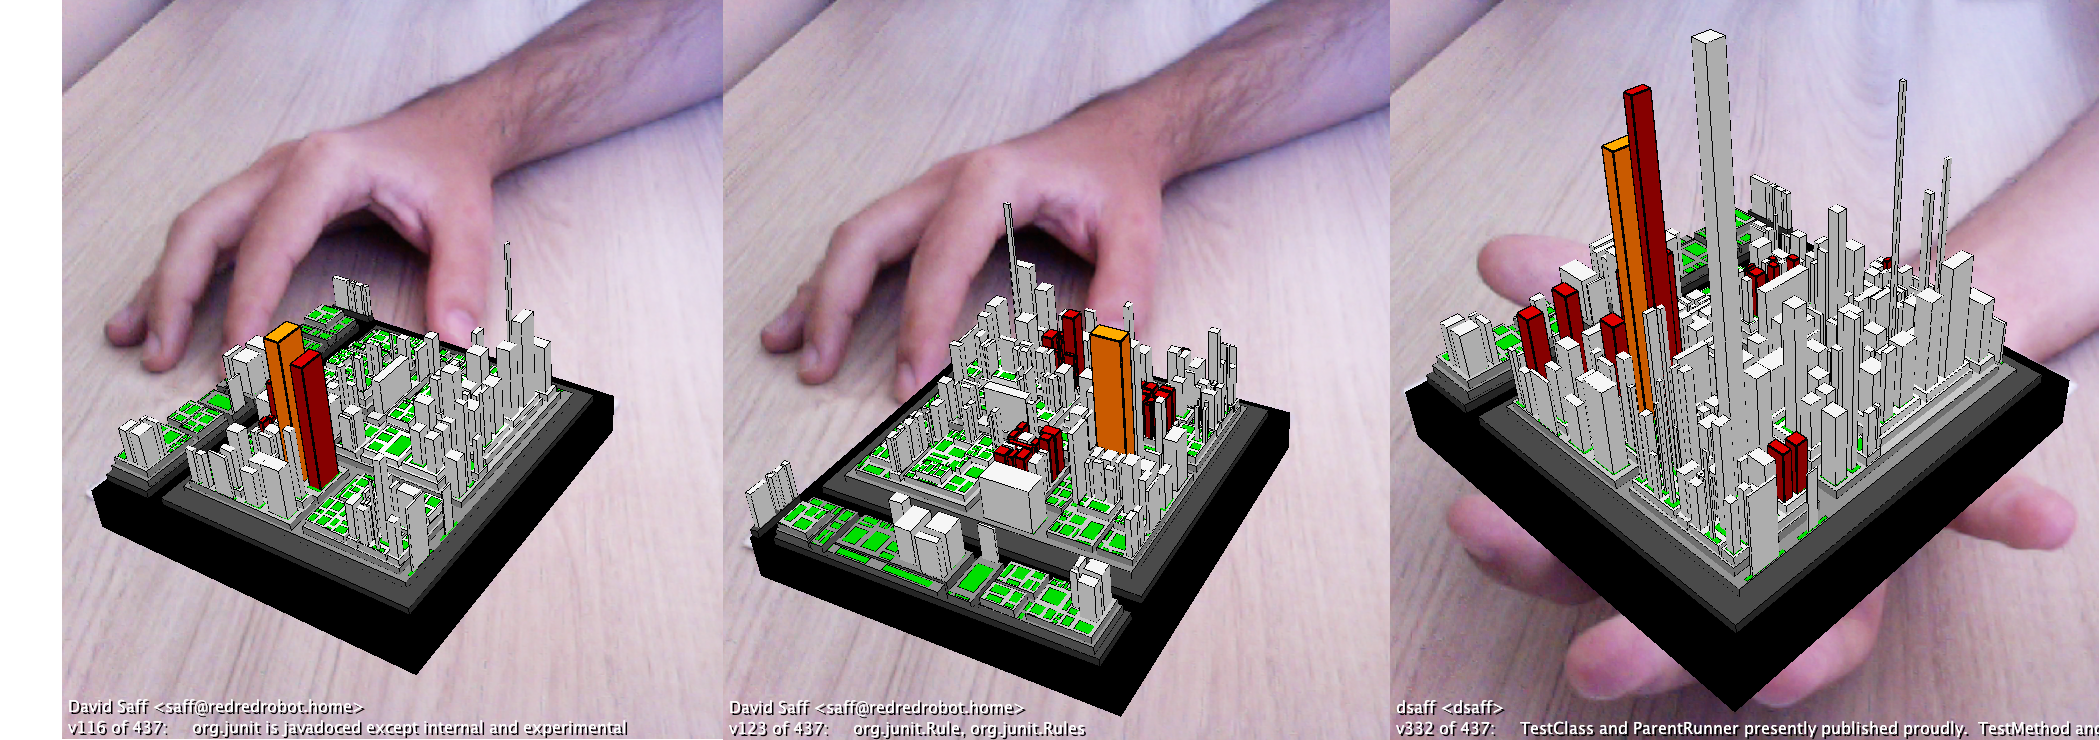
\includegraphics[width=0.8\textwidth, bb=14 14 2114 755]{./images/applications}
 % applications.eps: 0x0 pixel, 300dpi, 0.00x0.00 cm, bb=14 14 2114 755
 \caption{TO BE DEFINED...}
 \label{fig:TOBEDEFINED}
\end{figure*}

\textbf{Finding Skyscrapers.} In a software project, it is common to find classes which change a lot—the so called change-prone classes. In SkyscrapAR, they can be easily found as skyscrapers (see the orange building in Figure 3). Analog to the real concept, skyscrapers in our visualization are classes that concentrate a lot of the development effort. These classes deserve special attention, since they are more likely to be fault-prone \cite{nagappan:2005}. 

\textbf{Visualizing Scattering of Changes.} Source code management systems usually list packages and classes that were changed in each revision, but there is no visual information about the scattering of each commit transaction that generates a revision. This is easily done in SkycrapAR (see red buildings in Figure 3). Identifying scattered changes is important, as they represent modifications that impacted several systems modules, pointing out system-wide maintenance activities, such as refactoring’s or move operations among folders, or indicating that there are too many dependencies between software modules.

\textbf{Visualizing Classes Co-change.} Sometimes, classes have logical couplings even if they are not explicitly coupled to each other by their internal structural elements \cite{gall:1998}. Classes may be connected by means of implicit abstract elements related to the domain. For example, classes that are not structurally coupled but implement concerns that are strongly dependent at the requirements level. SkycrapAR provides information about the classes co-change by highlighting in red the classes that changed together in each revision (see Figure 3). 

\textbf{Finding God Classes.} A god class is a well-known code smell which refers to classes that perform too much work on its own. It breaks one of the basic principles of object-oriented design which states that a class should have one single responsibility. Also, implementing several responsibilities are more likely to undergo changes as much as the evolution history targets the responsibilities implemented by the class \cite{silva:2012}. SkyscrapAR helps developer to reason about god classes using the High Occupation of Territory metaphor - tall buildings occupying large areas.

\textbf{Identifying Populous Districts and City Centers.} Normally systems as cities have one or more neighborhoods with tall buildings and packages with no or very few green area - those areas are Populous Districts. This observation can be interpreted as the most touched parts of the system. If there is only a single well-defined populous district, we call it the City Center. Finding the city center (or other populous districts) may be useful to focus code inspection and testing on the most modified and possibly the most fault-prone parts of the system. It may also help to find refactoring opportunities on specific packages that suffered too many changes

\section{Final Remarks} \label{sec:finalRemarks}
This paper presented SkyscrapAR, an augmented reality visualization that employs the city metaphor to display information about the evolution of a software system. To the best of our knowledge, this is the first software visualization tool to employ augmented reality. In addition to describing SkyscrapAR, the paper shows how it can be used to support software comprehension tasks.

Currently, the tool has some limitations. In its current stage, only Java source code is supported, although it should be easy to add support for other languages. Also, it is limited to display one software system at a time, even if multiple markers are used. Finally, the user interaction still relies on the use of mouse and keyboard, which reduces the sense of immersion that characterizes augmented reality applications.

As future work, we intend to investigate interaction modes that dispense the use of mouse and keyboard. Our goal is to create a user interface that is intuitive, while discarding approaches that require expensive equipment such as virtual reality helmets and gloves. We also plan to make better use of colors in the visualization in order to display richer information. For instance, buildings can be painted in different colors to represent distinct crosscutting concerns implemented by them or, still, the developers who have contributed to the class. We plan to evaluate the tool with developers in academic or industrial settings. The evaluation should focus on usability and the effectiveness of the tool when used to support specific software comprehension tasks.

\section*{Acknowledgment}
The authors wish to thank Michele Lanza for encouraging this publication.